\documentclass{../industrial-development}
\graphicspath{{10-quality-assurance/}}

\title{Обеспечение качества ПО}
\author{Глазовский Александр, Совин Алексей}
\date{}

\begin{document}
	
	\begin{frame}
		\titlepage
	\end{frame}
	
	
	
	\section{Понятие качества ПО}
	\begin{frame} \frametitle{Понятие качества ПО}
		\begin{block}{}
			\alert{Качество программного обеспечения} --- это совокупность характеристик ПО, относящихся к его способности удовлетворять установленные и предполагаемые потребности пользователя
		\end{block}
		\begin{itemize}
			\item Функциональность (Functionality)
			\item Надежность (Reliability)
			\item Удобство использования (Usability)
			\item Эффективность (Efficiency)
			\item Удобство сопровождения (Maintainability)
			\item Портативность (Portability)
		\end{itemize}
	\end{frame}
	
	\begin{frame} \frametitle {Функциональность}
		\begin{block}{}
			\alert{Функциональность} --- способность ПО в определенных условиях решать задачи, нужные пользователям
		\end{block}
		\begin{itemize}
			\item Функциональная пригодность (suitability) --- способность решать нужный набор задач
			\item Точность (accuracy) --- способность выдавать нужные результаты
			\item Способность к взаимодействию (interoperability) --- способность взаимодействовать с набором других систем
			\item Соответствие стандартам и правилам (compliance)
			\item Защищенность (security) --- способность предотвращать неавторизированный доступ к данным и программам
		\end{itemize}
	\end{frame}
	
	\begin{frame} \frametitle {Надежность}
		\begin{block}{}
			\alert{Надежность} ---  способность  ПО  поддерживать  определенную  работоспособность в заданных условиях 
		\end{block}
		\begin{itemize}
			\item Зрелость, завершенность (maturity) --- величина, обратная частоте отказов ПО
			\item Устойчивость к отказам (fault tolerance) --- способность поддерживать заданный уровень работоспособности при отказах и нарушениях правил взаимодействия с окружением
			\item Способность к восстановлению (recoverability) --- способность восстанавливать определенный уровень работоспособности и целостность данных после отказа
			\item Соответствие стандартам надежности (reliability compliance)
		\end{itemize}
	\end{frame}
	
	\begin{frame} \frametitle {Удобство использования}
		\begin{block}{}
			\alert{Удобство использования} --- способность ПО быть удобным в обучении и использовании, а также привлекательным для пользователей 
		\end{block}
		\begin{itemize}
			\item Понятность (understandability) --- показатель, обратный к усилиям, затрачиваемым пользователями на восприятие основных понятий ПО
			\item Удобство обучения (learnability) --- показатель, обратный усилиям, затрачиваемым пользователями на обучение работе
			\item Удобство работы (operability) --- показатель, обратный усилиям, предпринимаемым пользователями для решения своих задач с помощью ПО
			\item Привлекательность (attractiveness) --- способность ПО быть привлекательным для пользователей
		\end{itemize}
	\end{frame}
	
	\begin{frame} \frametitle {Эффективность}
		\begin{block}{}
			\alert{Эффективность} --- способность ПО при заданных условиях обеспечивать необходимую работоспособность по отношению к выделяемым для этого ресурсам
		\end{block}
		\begin{itemize}
			\item Временная эффективность (time behaviour) --- способность ПО выдавать ожидаемые результаты и обеспечивать передачу необходимого объема данных за отведенное время
			\item Эффективность использования ресурсов (resource utilisation) --- способность решать нужные задачи с использованием определенных объемов ресурсов
		\end{itemize}
	\end{frame}
	
	\begin{frame} \frametitle {Удобство сопровождения}
		\begin{block}{}
			\alert{Удобство сопровождения} --- удобство проведения всех видов деятельности, связанных с сопровождение программ
		\end{block}
		\begin{itemize}
			\item Анализируемость (analyzability) --- удобство проведения анализа ошибок, а также удобство анализа необходимости изменений и их возможных последствий
			\item Удобство внесения изменений (changeability) --- показатель, обратный трудозатратам на выполнение необходимых изменений
			\item Стабильность (stability) --- показатель, обратный риску возникновения неожиданных эффектов при внесении необходимых изменений
		\end{itemize}
	\end{frame}	
	
	\begin{frame} \frametitle {Переносимость}
		\begin{block}{}
			\alert{Переносимость} --- способность ПО сохранять работоспособность при переносе из одного окружения в другое
		\end{block}
		\begin{itemize}
			\item Адаптируемость (adaptability) --- способность ПО приспосабливаться к различным окружениям без проведения для этого специальных действий
			\item Удобство установки (installability) --- способность ПО быть установленным в определенном окружении
			\item Способность к сосуществованию (coexistence) --- способность ПО сосуществовать с другими программами, деля с ними ресурсы
		\end{itemize}
	\end{frame}	
	
	\section{Понятие управления качеством}
	\begin{frame} \frametitle {Обеспечение качества}
		\begin{block}{}
			\alert{Обеспечение качества} --- это совокупность мероприятий, охватывающих все технологические этапы разработки, выпуска и эксплуатации ПО, предпринимаемых на разных стадиях жизненного цикла, для обеспечения требуемого уровня качества выпускаемого продукта	
		\end{block}
		\begin{itemize}
			\item Верификация --- процесс оценки системы или её компонентов с целью определения, удовлетворяют ли результаты текущего этапа разработки условиям, сформированным в начале этого этапа
			\item Валидация --- это определение соответствия разрабатываемого ПО ожиданиям и потребностям пользователя, требованиям к системе
		\end{itemize}
	\end{frame}	
	
	\begin{frame} \frametitle{Иерархия процессов QA}
		\centerline{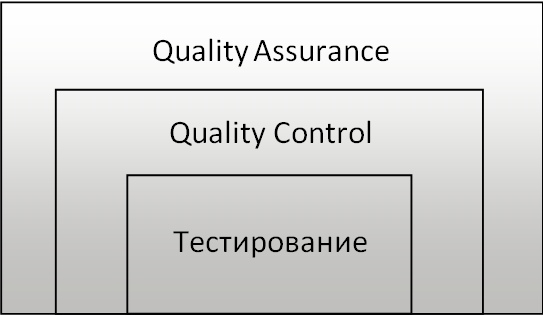
\includegraphics[height=0.7\textheight]{QA_QC2.png}}
	\end{frame}
	
	\begin{frame} \frametitle{Иерархия процессов QA}
		\begin{itemize}
			\item Quality Assurance обеспечивает правильность и предсказуемость процесса 
			
			\item Quality Control --- гарантирует соответствие требованиям (поиск ошибок и их устранение).
			
			\item Тестирование --- это сбор статистических данных и внесение их в документы, созданные в рамках QC-процесса.
		\end{itemize}
	\end{frame}
	
	\begin{frame} \frametitle{Иерархия процессов QA}
		\begin{block}{}
			\centerline{	Cравнение процессов	}
		\end{block}
		\centerline{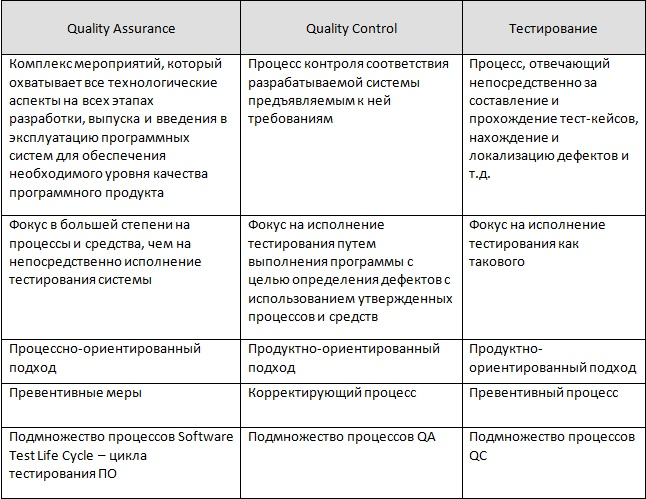
\includegraphics[height=0.7\textheight]{QA_QC.png}}
	\end{frame}
		
	\section{Процессы QA}
	\begin{frame} \frametitle{Обзор требований и документации продукта}
		\begin{block}{}
			\alert{Цель} --- анализ системной архитектуры и технологий на предмет расхождений
		\end{block}
		\begin{itemize}
			\item Полнота (completeness)
			\item Избыточность (redundancies)
			\item Ясность (clarity)
			\item Последовательность (consistency)
			\item Исполняемость (executability)
			\item Проверяемость (verifiability)
		\end{itemize}
	\end{frame}
	
	\begin{frame} \frametitle{Дымовое тестирование}
		\begin{block}{}
			\alert{Дымовое тестирование (Smoke testing)} --- короткий цикл тестов, подтверждающий, что после сборки приложение выполняет основные функции
		\end{block}
	\end{frame}
	
	\begin{frame} \frametitle{Интеграционное тестирование}
		\begin{block}{}
			\alert{Интеграционное тестирование (Integration testing)} --- цикл тестов, подтверждающий, что различные компоненты продукта работают, как единая система
		\end{block}
		\begin{itemize}
			\item Проверяется взаимодействие между компонентами системы
			\item Проверяется взаимодействие между разными системами
		\end{itemize}
	\end{frame}
	
	\begin{frame} \frametitle{Тестирование проиводительности}
		\begin{block}{}
			\alert{Тестирование проиводительности (Performance testing)} --- тестирование, направленное на определение масштабируемости приложения под нагрузкой
		\end{block}
		\begin{itemize}
			\item Измерение времени выполнения выбранных операций при определенных интенсивностях выполнения этих операций
			\item Определение количества пользователей, одновременно работающих с приложением
			\item Определение границ приемлемой производительности при увеличении нагрузки
			\item Исследование производительности на высоких, предельных, стрессовых нагрузках
		\end{itemize}
	\end{frame}
	
	\begin{frame} \frametitle{Тестирование безопасности}
		\begin{block}{}
			\alert{Тестирование безопасности (Security testing)} --- тестирование, используемое для проверки безопасности системы
		\end{block}
		\begin{itemize}
			\item Конфиденциальность
			\item Целостность
			\item Доступность
		\end{itemize}
	\end{frame}
	
	\begin{frame} \frametitle{Кросс-платформенное тестирование}
		\begin{block}{}
			\alert{Кросс-платформенное тестирование (Cross-platform testing)} --- тестирование, проверяющее, что приложение работает одинаково на разных платформах
		\end{block}
	\end{frame}
	
	\begin{frame} \frametitle{Регрессионное тестирование}
		\begin{block}{}
			\alert {Регрессионное тестирование (Regression testing)} --- вид тестирования направленный на проверку изменений для подтверждения, что существующая ранее функциональность работает как прежде
		\end{block}
	\end{frame}
	
	\begin{thebibliography}{99}
		\bibitem{SQA-Galin} Galin, Daniel, Software quality assurance: from theory to implementation / Daniel Galin, 2004."--- 590с.: ил.
	\end{thebibliography}
	
\end{document}